% Options for packages loaded elsewhere
\PassOptionsToPackage{unicode}{hyperref}
\PassOptionsToPackage{hyphens}{url}
%
\documentclass[
]{article}
\usepackage{amsmath,amssymb}
\usepackage{lmodern}
\usepackage{iftex}
\ifPDFTeX
  \usepackage[T1]{fontenc}
  \usepackage[utf8]{inputenc}
  \usepackage{textcomp} % provide euro and other symbols
\else % if luatex or xetex
  \usepackage{unicode-math}
  \defaultfontfeatures{Scale=MatchLowercase}
  \defaultfontfeatures[\rmfamily]{Ligatures=TeX,Scale=1}
\fi
% Use upquote if available, for straight quotes in verbatim environments
\IfFileExists{upquote.sty}{\usepackage{upquote}}{}
\IfFileExists{microtype.sty}{% use microtype if available
  \usepackage[]{microtype}
  \UseMicrotypeSet[protrusion]{basicmath} % disable protrusion for tt fonts
}{}
\makeatletter
\@ifundefined{KOMAClassName}{% if non-KOMA class
  \IfFileExists{parskip.sty}{%
    \usepackage{parskip}
  }{% else
    \setlength{\parindent}{0pt}
    \setlength{\parskip}{6pt plus 2pt minus 1pt}}
}{% if KOMA class
  \KOMAoptions{parskip=half}}
\makeatother
\usepackage{xcolor}
\usepackage[margin=1in]{geometry}
\usepackage{graphicx}
\makeatletter
\def\maxwidth{\ifdim\Gin@nat@width>\linewidth\linewidth\else\Gin@nat@width\fi}
\def\maxheight{\ifdim\Gin@nat@height>\textheight\textheight\else\Gin@nat@height\fi}
\makeatother
% Scale images if necessary, so that they will not overflow the page
% margins by default, and it is still possible to overwrite the defaults
% using explicit options in \includegraphics[width, height, ...]{}
\setkeys{Gin}{width=\maxwidth,height=\maxheight,keepaspectratio}
% Set default figure placement to htbp
\makeatletter
\def\fps@figure{htbp}
\makeatother
\setlength{\emergencystretch}{3em} % prevent overfull lines
\providecommand{\tightlist}{%
  \setlength{\itemsep}{0pt}\setlength{\parskip}{0pt}}
\setcounter{secnumdepth}{-\maxdimen} % remove section numbering
\usepackage{titling}
\pretitle{
  \begin{center}
  \huge
  \setmainfont{Georgia}
  
\includegraphics[width=4cm,height=6cm]{../_extensions/cityforwardcollective/img/logo.png}\\[\bigskipamount]
}
\posttitle{\end{center}}
\posttitle{\end{center}}
\usepackage{booktabs}
\usepackage{longtable}
\usepackage{array}
\usepackage{multirow}
\usepackage{wrapfig}
\usepackage{float}
\usepackage{colortbl}
\usepackage{pdflscape}
\usepackage{tabu}
\usepackage{threeparttable}
\usepackage{xcolor}
\usepackage{soul}
\usepackage{graphicx}
\usepackage{fancyhdr}
\pagestyle{fancy}
\rhead{
\includegraphics[width = .15\textwidth]{../_extensions/cityforwardcollective/img/logo.png}}
\usepackage{booktabs}
\usepackage{longtable}
\usepackage{array}
\usepackage{multirow}
\usepackage{wrapfig}
\usepackage{float}
\usepackage{colortbl}
\usepackage{pdflscape}
\usepackage{tabu}
\usepackage{threeparttable}
\usepackage{threeparttablex}
\usepackage[normalem]{ulem}
\usepackage{makecell}
\usepackage{xcolor}
\ifLuaTeX
  \usepackage{selnolig}  % disable illegal ligatures
\fi
\IfFileExists{bookmark.sty}{\usepackage{bookmark}}{\usepackage{hyperref}}
\IfFileExists{xurl.sty}{\usepackage{xurl}}{} % add URL line breaks if available
\urlstyle{same} % disable monospaced font for URLs
\hypersetup{
  pdftitle={School Breakdown for State Legislators},
  hidelinks,
  pdfcreator={LaTeX via pandoc}}

\title{School Breakdown for State Legislators}
\usepackage{etoolbox}
\makeatletter
\providecommand{\subtitle}[1]{% add subtitle to \maketitle
  \apptocmd{\@title}{\par {\large #1 \par}}{}{}
}
\makeatother
\subtitle{Kalan Haywood---Assembly District 16}
\author{}
\date{\vspace{-2.5em}}

\begin{document}
\maketitle

{
\setcounter{tocdepth}{3}
\tableofcontents
}
\newpage

\hypertarget{district-16-overview}{%
\section{District 16 Overview}\label{district-16-overview}}

\vspace{.25in}

\begin{center}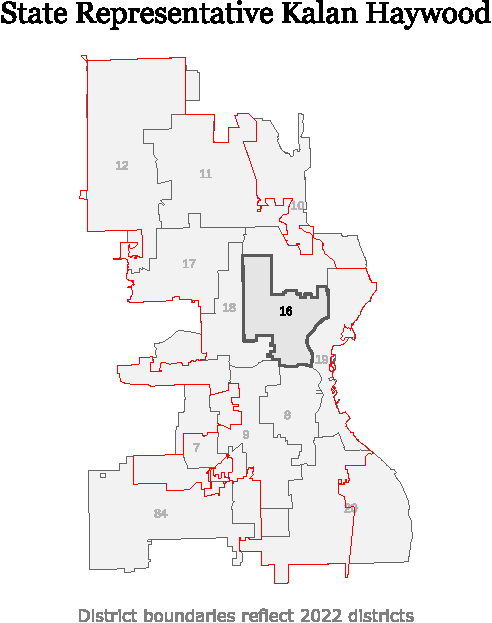
\includegraphics{haywood_assembly_files/figure-latex/unnamed-chunk-1-1} \end{center}

\newpage

\begin{center}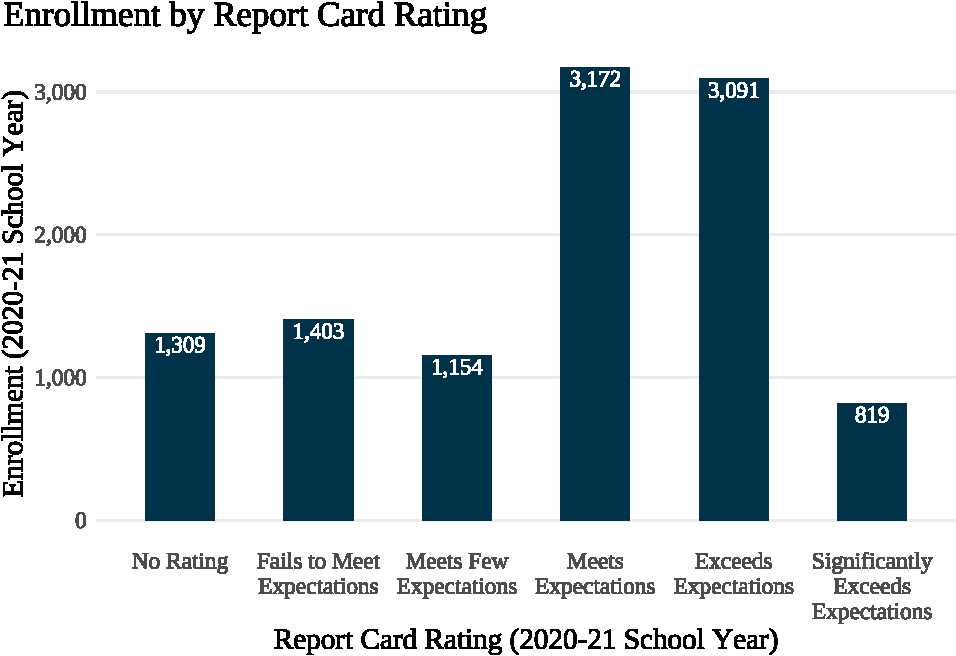
\includegraphics[width=0.85\linewidth]{haywood_assembly_files/figure-latex/unnamed-chunk-2-1} \end{center}

\begin{center}\includegraphics[width=0.85\linewidth]{haywood_assembly_files/figure-latex/unnamed-chunk-3-1} \end{center}

\newpage

\hypertarget{list-of-schools-in-district-16}{%
\section{List of Schools in District
16}\label{list-of-schools-in-district-16}}

\begingroup\fontsize{8}{10}\selectfont

\begin{longtable}[t]{>{\raggedright\arraybackslash}p{10em}ll>{\raggedright\arraybackslash}p{10em}r}
\caption{\label{tab:unnamed-chunk-4}School List with 2020-21 Report Cards}\\
\toprule
School & Sector & Grades & Report Card Rating & Report Card Score\\
\midrule
\cellcolor{gray!6}{Alliance School of Milwaukee} & \cellcolor{gray!6}{Instrumentality Charter} & \cellcolor{gray!6}{9-12} & \cellcolor{gray!6}{Alternate Rating - Needs Improvement} & \cellcolor{gray!6}{NA}\\
Auer Avenue Elementary & Traditional Public & K-5 & Meets Few Expectations & 53.8\\
\cellcolor{gray!6}{Brown Street Academy} & \cellcolor{gray!6}{Traditional Public} & \cellcolor{gray!6}{K-5} & \cellcolor{gray!6}{Meets Few Expectations} & \cellcolor{gray!6}{55.7}\\
Carver Academy & Traditional Public & K-8 & Exceeds Expectations & 72.9\\
\cellcolor{gray!6}{Clara Mohammed School} & \cellcolor{gray!6}{Private} & \cellcolor{gray!6}{K-12} & \cellcolor{gray!6}{NR-DATA} & \cellcolor{gray!6}{NA}\\
\addlinespace
Clarke Street Elementary & Traditional Public & K-8 & Meets Expectations & 61.2\\
\cellcolor{gray!6}{Cross Trainers Academy} & \cellcolor{gray!6}{Private} & \cellcolor{gray!6}{K-12} & \cellcolor{gray!6}{Meets Expectations} & \cellcolor{gray!6}{69.2}\\
Elm Creative Arts Elementary & Traditional Public & K-5 & Fails to Meet Expectations & 33.2\\
\cellcolor{gray!6}{Franklin Elementary} & \cellcolor{gray!6}{Traditional Public} & \cellcolor{gray!6}{K-8} & \cellcolor{gray!6}{Meets Expectations} & \cellcolor{gray!6}{62.7}\\
Golda Meir School & Traditional Public & K-12 & Exceeds Expectations & 74.3\\
\addlinespace
\cellcolor{gray!6}{Grant Gordon Learning Center} & \cellcolor{gray!6}{Traditional Public} & \cellcolor{gray!6}{K-5} & \cellcolor{gray!6}{NA} & \cellcolor{gray!6}{NA}\\
Highland Community School & Non-Instrumentality Charter & K-8 & Exceeds Expectations & 70.4\\
\cellcolor{gray!6}{Holmes Elementary} & \cellcolor{gray!6}{Traditional Public} & \cellcolor{gray!6}{K-8} & \cellcolor{gray!6}{Meets Expectations} & \cellcolor{gray!6}{60.7}\\
Hope Christian School: Prima & Private & K-8 & Exceeds Expectations & 76.5\\
\cellcolor{gray!6}{Jackson Elementary} & \cellcolor{gray!6}{Traditional Public} & \cellcolor{gray!6}{K-5} & \cellcolor{gray!6}{Fails to Meet Expectations} & \cellcolor{gray!6}{26.0}\\
\addlinespace
King International Baccalaureate Middle & Traditional Public & 6-8 & Meets Few Expectations & 49.4\\
\cellcolor{gray!6}{Metcalfe Elementary} & \cellcolor{gray!6}{Traditional Public} & \cellcolor{gray!6}{K-8} & \cellcolor{gray!6}{Meets Expectations} & \cellcolor{gray!6}{61.2}\\
Milwaukee College Preparatory School -- Lloyd Street & Non-Instrumentality Charter & K-8 & Meets Expectations & 61.6\\
\cellcolor{gray!6}{Milwaukee College Preparatory School: Lola Rowe North Campus} & \cellcolor{gray!6}{Non-Instrumentality Charter} & \cellcolor{gray!6}{K-8} & \cellcolor{gray!6}{Exceeds Expectations} & \cellcolor{gray!6}{76.3}\\
Milwaukee County Youth Education Center & Traditional Public & 6-12 & Alternate Rating - Satisfactory Progress & NA\\
\addlinespace
\cellcolor{gray!6}{Next Door Charter} & \cellcolor{gray!6}{Non-Instrumentality Charter} & \cellcolor{gray!6}{K-5} & \cellcolor{gray!6}{NA} & \cellcolor{gray!6}{NA}\\
North Division High & Traditional Public & 9-12 & Fails to Meet Expectations & 12.6\\
\cellcolor{gray!6}{NOVA-Northwest Opportunities Vocational Academy} & \cellcolor{gray!6}{Partnership} & \cellcolor{gray!6}{9-12} & \cellcolor{gray!6}{Alternate Rating - Needs Improvement} & \cellcolor{gray!6}{NA}\\
Pathways High & 2r/2x Charter & 9-12 & Meets Expectations & 61.6\\
\cellcolor{gray!6}{Penfield Montessori Academy} & \cellcolor{gray!6}{2r/2x Charter} & \cellcolor{gray!6}{K-5} & \cellcolor{gray!6}{Alternate Rating - Satisfactory Progress} & \cellcolor{gray!6}{NA}\\
\addlinespace
Project STAY-Supporting Teachers and Youth & Traditional Public & 9-12 & Alternate Rating - Needs Improvement & NA\\
\cellcolor{gray!6}{Riverwest Elementary} & \cellcolor{gray!6}{Traditional Public} & \cellcolor{gray!6}{K-5} & \cellcolor{gray!6}{Meets Few Expectations} & \cellcolor{gray!6}{51.1}\\
Roosevelt Middle & Traditional Public & 6-8 & Meets Expectations & 62.3\\
\cellcolor{gray!6}{Saint Marcus Lutheran School} & \cellcolor{gray!6}{Private} & \cellcolor{gray!6}{K-8} & \cellcolor{gray!6}{Significantly Exceeds Expectations} & \cellcolor{gray!6}{91.6}\\
Shalom High & Partnership & 9-12 & Alternate Rating - Needs Improvement & NA\\
\addlinespace
\cellcolor{gray!6}{Siefert Elementary} & \cellcolor{gray!6}{Traditional Public} & \cellcolor{gray!6}{K-5} & \cellcolor{gray!6}{Meets Expectations} & \cellcolor{gray!6}{62.4}\\
Siloah Lutheran School & Private & K-8 & Fails to Meet Expectations & 41.1\\
\cellcolor{gray!6}{Starms Discovery} & \cellcolor{gray!6}{Traditional Public} & \cellcolor{gray!6}{K-8} & \cellcolor{gray!6}{Meets Expectations} & \cellcolor{gray!6}{66.6}\\
Starms Early Childhood & Traditional Public & K-5 & NA & NA\\
\cellcolor{gray!6}{Wisconsin Conservatory of Lifelong Learning} & \cellcolor{gray!6}{Traditional Public} & \cellcolor{gray!6}{K-12} & \cellcolor{gray!6}{Fails to Meet Expectations} & \cellcolor{gray!6}{39.5}\\
\bottomrule
\end{longtable}
\endgroup{}

\end{document}
